\section{iPhoneで他のアプリと連携}
こんにちは。会社や趣味でiPhoneアプリを作ったりしている@mtgtoです。
二回目の登場でございます。
今までに複数のiPhoneアプリを作っているのですが、アプリ間の連携をやったりしたことがありました。
AndroidのServiceのような仕組みがないiOSではアプリ間の連携はあまり得意ではないようですが、気になったので色々と調べたり試したりしてみました。

\subsection{諸注意}
\begin{itemize}
  \item この話はApp Storeのレビューを受けてない話が含まれるので、実際に使用する際は自己責任でお願い致します。
  \item 動作確認にはLion 10.7.4 on MacBook Air (2011), Xcode 4.3.3, iOS 5.1.1 on iPhone 4を使用しています。
  \item 実行に使用したソースコードは http://github.com/mtgto/c82 から見ることができます。
\end{itemize}
\subsection{NSURL形式}
まず最初に紹介するのはAppleによる公式で用意されている由緒正しいプロセス間のデータのやり取りを行う方法です。

自分のアプリオリジナルのカスタムURLスキーム(URLのプロトコル部分)をInfo.plistに書いておき、
そのプロトコルを使ったURLを開くことで別のアプリの起動&URLにデータを含めることでデータの受け渡しをすることができます。

このカスタムURLスキームを使う方法は、iOS 4.1までのAPIでは起動アプリが何かを判定できません。
\begin{itembox}{起動URL取得 (iOS 4.1まで)}
- (BOOL)application:(UIApplication *)application handleOpenURL:(NSURL *)url
\end{itembox}
iOS 4.2以上では起動元アプリの情報が取れるAPIが提供され、上記の物は非推奨となりました。
\begin{itembox}{起動URL取得 (iOS 4.2以降)}
- (BOOL)application:(UIApplication *)application openURL:(NSURL *)url sourceApplication:(NSString *)sourceApplication annotation:(id)annotation
\end{itembox}
iPhone Simulatorや実機上でURLスキーマによるアプリの起動を試してみるとわかりますが、sourceApplicationには起動したアプリのバンドルIDが来るので、
自分以外のアプリからの起動であればNOを返すことにより自分が許可するアプリからのみ要求された動作を行うことが可能です
(他のアプリから起動させないことは不可能)。
特にUIWebViewを多用しているウェブアプリからネイティブのコードを呼び出すときにはこのカスタムURLスキームの仕組みを使用することが多いと思いますが、
その場合も自分のアプリのバンドルIDから起動されているかのチェックを行うようにしましょう。

\begin{figure}
  \centering
  \fbox{
    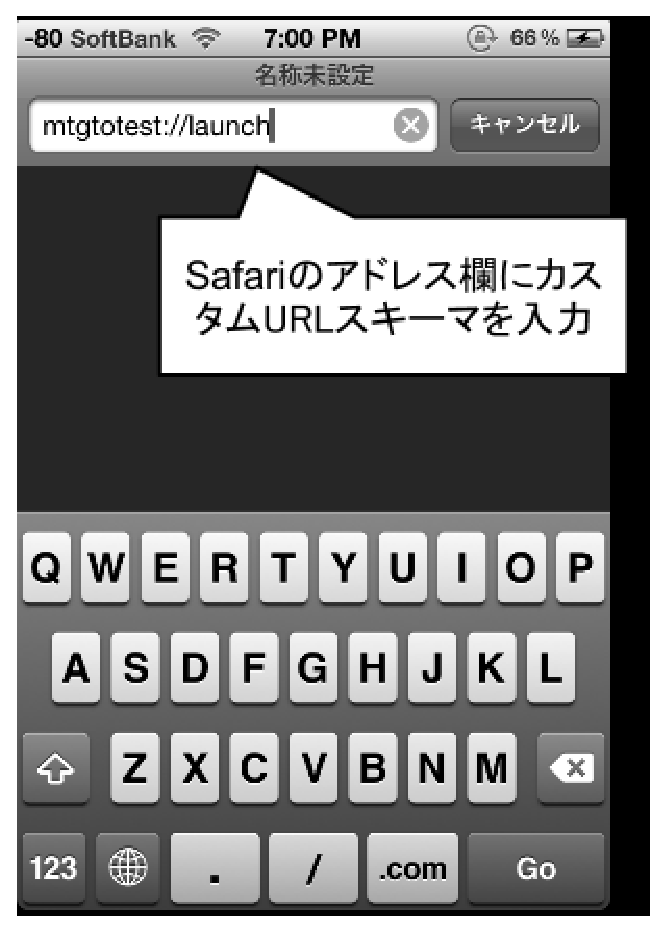
\includegraphics[width=9cm,clip]{goto-pedia/img/url-launch.eps}
  }
  \caption{カスタムURLで自アプリを起動する}
\end{figure}


\subsubsection{受け取ったクエリをパースする方法}
URL形式でデータを渡すときにはURLのクエリ部分を辞書のように使うことが一般的である気がします(実経験より)。
以下どこにでもあるようなURLパースの処理(こういうのをNSStringのカテゴリとして拡張して自分のプロジェクトにおいておくといいと思う)。
\begin{lstlisting}{language=[objective]c;caption=起動URLクエリをパースする方法}
for (NSString* parameterString in [queryString componentsSeparatedByString:@"&"]) {
  NSArray* parameterArray = [parameterString componentsSeparatedByString:@"="];
  if ([parameterArray count] != 2) {
	NSLog(@"Invalid parameter: %@", parameterString);
	continue;
  }
  NSString* parameterKey = [(NSString*)[parameterArray objectAtIndex:0]
	stringByReplacingPercentEscapesUsingEncoding:NSUTF8StringEncoding];
  NSString* parameterValue = [(NSString*)[parameterArray objectAtIndex:1]
	stringByReplacingPercentEscapesUsingEncoding:NSUTF8StringEncoding];
  NSLog(@"key=%@, value=%@", parameterKey, parameterValue);
}
\end{lstlisting}
例えば\htmladdnormallinkfoot{Facebook iOS SDK}{https://developers.facebook.com/docs/mobile/ios/build/}ではこの仕組みを利用して、自作アプリからFacebookアプリを呼び出してユーザ認証などを行うことができます。

またDefault-myscheme.png(myschemeはURLスキーマ)を起動時のスプラッシュ画面と同じ大きさで作成しておくと、
通常起動時とURLからの起動時で別の画像を使うことができます。

\subsection{ソケット通信}
先のNSURL形式では情報を通知するために別アプリを一度フォアグラウンドにする必要があります。
そのため、細かい情報のやり取りをしたい場合にはNSURLは向いていないことになります。
プロセスがバックグラウンドにいるときに
バックグラウンドで実行しているアプリケーションは通常だと10分までしか処理を行なってくれず、
それを超えるとOSによってプロセスが強制的に終了されてしまいます。

ここでは\htmladdnormallinkfoot{CocoaAsyncSocket}{https://github.com/robbiehanson/CocoaAsyncSocket}を使ってみましょう。
GCD版とRunLoop版の二種類がありますが、iOSの場合ハードウェアリソースに限りがあるので、どちらでも構わないと思っています。
今回はGCD版でサーバとクライアントを作ってみました。

TCP通信であれば難なく接続することができますが、当然他のアプリにバインドされてしまうこともあるのでポートを固定にしないよう実装しましょう。
その場合使用するポートをどうやって相手のアプリに渡すか考えなければなりません。

またバックグラウンドで受信するためにはバックグラウンドタスクとして登録しておく必要があります。

\subsection{NSNotifactionCenter}
Mac OS Xの場合、NSDistributedNotificationCenterを使って他のアプリケーション間でメッセージのやり取りをすることができます。
ですがiOSにはありません。
\subsubsection{メッセージを受ける側の処理}
\begin{itemize}
  \item \htmladdnormallinkfoot{CPDistributedMessagingCenter.h}{https://github.com/kennytm/iphone-private-frameworks/blob/master/AppSupport/CPDistributedMessagingCenter.h}をプロジェクトに追加する。
  \item CPDistributedMessagingCenter\#centerNamedで自分の通知センターを作る
  \item CPDistributedMessagingCenter\#registerForMessageNameで通知したいメッセージとセレクタを登録
\end{itemize}

\subsubsection{メッセージを送る側の処理}
\begin{itemize}
  \item CPDistributedMessagingCenter.hをプロジェクトに追加する
  \item CPDistributedMessagingCenter\#centerNamedで自分の通知センターを作る
  \item CPDistributedMessagingCenter\#sendMessageName:userInfo:で送信する
\end{itemize}

ただしCPDistributedMessagingCenterはプライベートAPIなので、App Storeに出すときにはほぼ間違いなくリジェクト食らうと思います。
とはいえ便利なので個人のiPhoneで楽しむか、jailbreak環境で楽しむくらいがいいですね。

\subsection{共有メモリ形式}
iOSにはサンドボックス機構があり、他プロセスのメモリに直接アクセスすることは出来ません。
そこで(POSIXの)共有メモリを使ってプロセス間で読み書きを行うということを考えました。

方法としては、POSIXのshm\_open関数でファイルディスクリプタのように開き、mmapすることでメモリとして扱うことができます。

\subsection{ファイル}
\htmladdnormallinkfoot{iOS アプリケーションプログラミングガイド}{https://developer.apple.com/jp/devcenter/ios/library/documentation/iPhoneAppProgrammingGuide.pdf}によると
アプリケーション(および環境設定を含むデータ)はサンドボックスでデータが保護されており、
他のアプリからアクセスすることができない、とあります。

ものは試しにと実際にあるアプリでファイルの書き込みを行い、そのファイルを他のアプリからアクセスするプログラムを作って実際にやってみたところ、
iOS Simulatorでは
``~/Library/Application Support/iPhone Simulator/5.1/Applications/(UUID)/''に書きだされ、他のアプリからパスを指定すれば開くことができましたが(サンドボックスの保護がされていない)、実機では
``The operation couldn't be completed. Operation not permitted''というエラー(NSErrorのdescription)が発生して開けませんでした。

\subsection{NSUserDefaults \& KeyChain Access}
NSUserDefaultsの説明に「他のアプリの設定へのaddSuiteNamed:を使ったアクセスは取得できないよ」とあります。

一方Keychainは\htmladdnormallinkfoot{同一プロビジョニングであれば他のアプリの設定項目を見ることができる}{http://cocoadays.blogspot.jp/2011/02/ios-keychain-services.html}との話があるので、自分のアプリであればキーチェーンを使ったデータの共有ができるようです。

\subsection{脱線:fork}
あまり関係ないのですが、iPhoneでforkすればAndroidのServiceのようなことができるのではないかと思って試してみました。
forkというのは自分のプロセスを複製して新しいプロセスを作るPOSIXの関数です。
試しにこんなコードを書いてみました:
\begin{lstlisting}{language=c, caption=fork}
int pid = fork();
if (pid < 0) {
	NSLog(@"fork failed");
} else if (pid == 0) {
	for (int i=0; i<1000; i++) {
		NSLog(@"%d", i);
		sleep(1);
	}
} else {
	int retVal = UIApplicationMain(argc, argv, nil, nil);
	[pool release];
	return retVal;
}
\end{lstlisting}
フレームワークの追加をすることなく、コンパイル&リンクには成功しました。

実際に動かしてみたところiOS Simulatorでは動作しましたが、実機だとエラーが帰ってきました。
残念ながらforkはできないようです。

\subsection{終わりに}
一つのバックグラウンドアプリを立ち上げておき、他のアプリで利用するのが難しいことが、iOSとAndroidで大きく違うところだと個人的には感じています。
今回は試しませんでしたが、OSが提供しているデータ共有のAPI、例えばカレンダーや写真を使う方法もあるでしょう。

それではまたどこかでお会いしましょう。またねー。
